
\chapter{Introduction}

\section{LibALF Basics}
		The \libalf library is an actively developed, stable, and extensively-tested library for learning finite state machines. It unifies different kinds of learning techniques into a single flexible, easy-to-extend, open source library with a clear and easy-to-understand user interface.
		\paragraph{}	
		The \libalf Library provides a wide range of \online and \offline algorithms for learning Deterministic (DFA) and Non Determinisitc Finite Automaton (NFA). \online algorithm is a technique where the hypothesis is built by understanding the classification (whether accepted or rejected) of queries asked to some kind of a \teacher.  While, an \offline algorithm builds an apposite hypothesis from a set of classified examples that were passively provided to it. As of \today, the library contains seven such algorithms implemented in it which are listed in Table \ref{algtables}.

		\begin{table}
		\centering
		\begin{tabular}[c]{lcr}
		\toprule[1pt]
			Online Algorithms & Offline Algorithms \\	
		\midrule
			Angluin's L [2] (two variants) & Biermann [3] \\
			NL [4] & RPNI [13] \\
			Kearns / Vazirani [10] & DeLeTe2 [6]\\
		\bottomrule[1pt]
		\end{tabular}
		\caption{List of Algorithms Implemented}
		\label{algtables}
		\end{table}
		
	  \paragraph{}	
		The central aim of \libalf Library is to provide significant advantages through potential features to the user. Our design of the tool primarily focuses on offering high flexibility and extensibility. 
	  \paragraph{}	
		Flexibility is realized through two essential features the library offers. The first being the support for switching easily between learning algorithms and information sources, which allows the user to experiment with different learning techniques. The second being the versatility of the tool. Since it is available in both \cpp and \java (using the Java Native Interface), it can be used in all familiar operating systems (Windows, Linux and MacOS in 32- and 64-bit). In addition, the dispatcher implements a network based client-server architecture, which allows one to run \libalf not only in local environment but also remotely, e.g., on a high performance machine.
		\paragraph{}
		In contrast, the goal of extensibility is to provide easy means to augment the library. This is mainly achieved by \libalf's easy-to-extend design and distributing \libalf freely as open source code. Its modular design and its implementation in \cpp makes it the ideal platform for adding and engineering further, other efficient learning algorithms for new target models (e.g., B�chi automata, timed automata, or probabilistic automata). 
		\paragraph{}
		Other pivotal features of the library include, ability to change the \alphsize during the learning process, extensive logging facilities, domain-based optimizations via so-called normalizers and filters, GraphViz visualization.
		
		
\section{Conceptual Details}

	The \libalf consists of four main components, the Learning Algorithm, the Knowledgebase, Filters \& Normalizers and Logger \& Statistics. Figure \ref{fig:components} shows a characteristic view of the these components. Our implemention of these components allows for plug and play usage.

\begin{figure}[h]
  \centering
  \subfloat[Algorithms]{\label{fig:alg}
\includegraphics[width=0.35\textwidth,scale=0.3]{Images/1.png}}  \hspace{30pt}           
  \subfloat[Knowledgebase]{\label{fig:base}
\includegraphics[width=0.3\textwidth]{Images/2.png}}\\
  \subfloat[Filter \& Normalizer]{\label{fig:filter}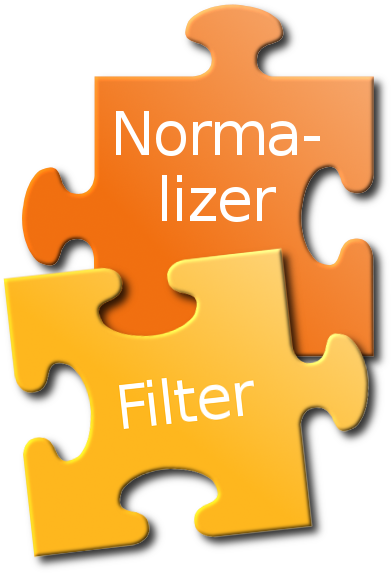
\includegraphics[width=0.27\textwidth]{Images/3.png}} \hspace{30pt}
  \subfloat[Logger \& Statistics]{\label{fig:logger}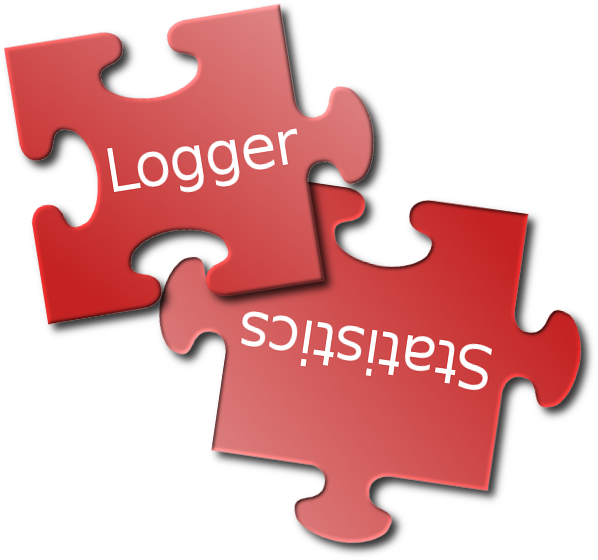
\includegraphics[width=0.35\textwidth]{Images/4.png}}
  \caption{Components of LibALF}
  \label{fig:components}
\end{figure} 
	
\subsection{The Knowledgebase}

	The knowledgebase is an efficient storage for language information that accumulates every word and its associated classification. It allows storage of values of arbitrary types and in the forthcoming sections we will describe its implementation where a word is stored as a list or array of \texttt{Integers}.
	It forms the fundamental source of information for a learning algorithm. Using an external storage for the knowledgebase has the advantage of it being independent of the choice of the learning algorithm. This enables interchanging of learning algorithms on the basis of same knowledge available. 
	
\begin{figure}[h]
	\centering
	\subfloat{\label{fig:baseandalg}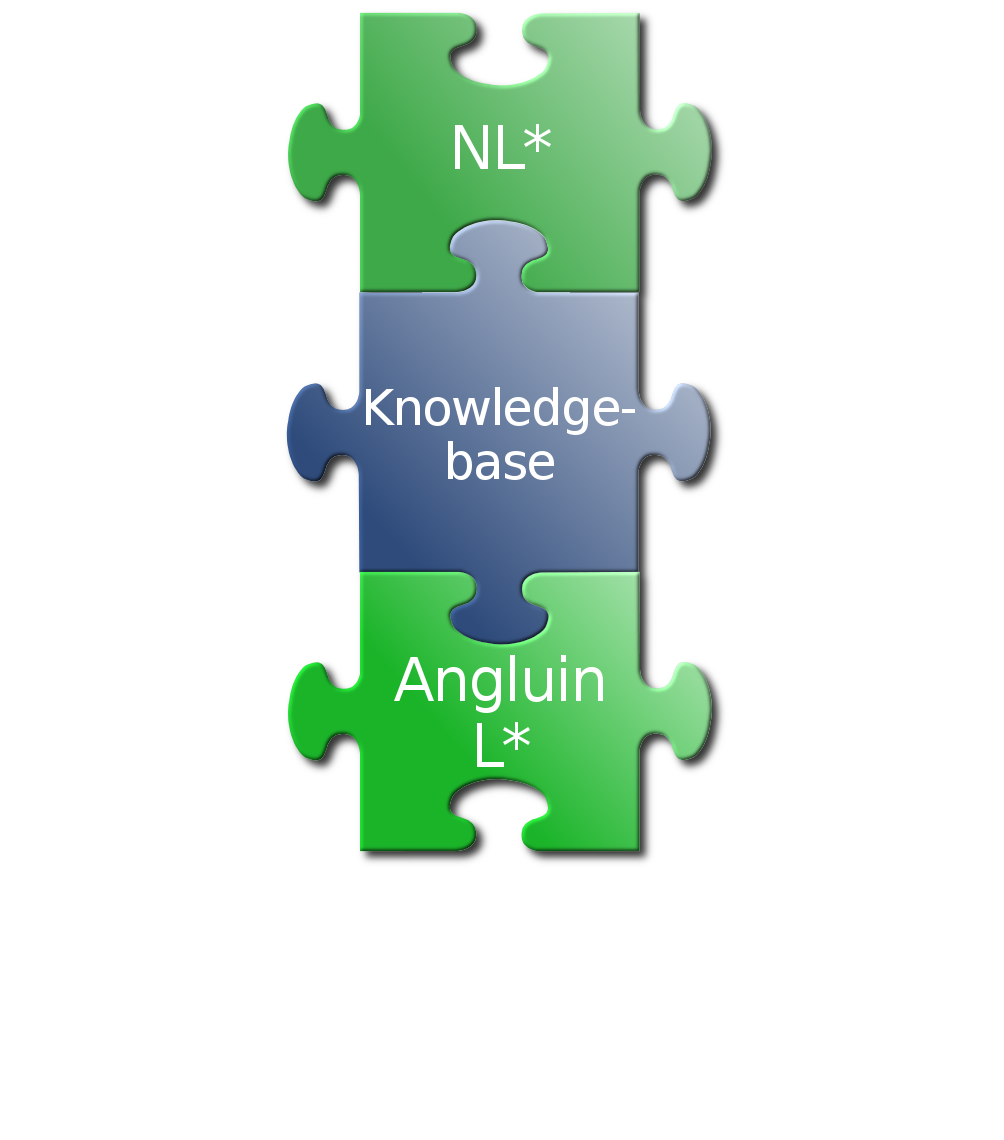
\includegraphics[width=0.5\textwidth]{Images/combined3.png}}
	\subfloat{\label{fig:basealgfilt}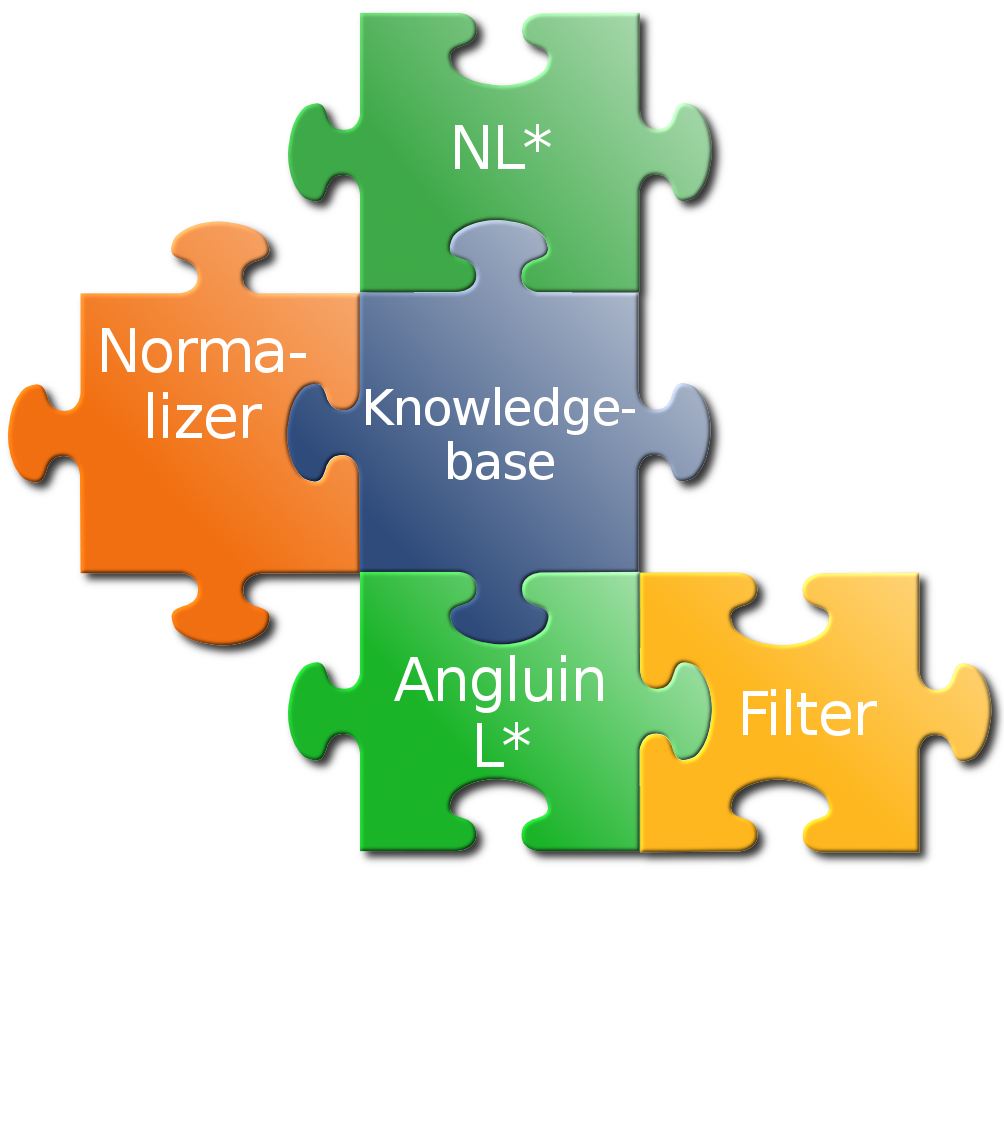
\includegraphics[width=0.5\textwidth]{Images/combined5.png}}
	\caption{Pictorial Representation of Plug and Play support}
	\label{fig:plug}
\end{figure}

\subsection{Learning Algorithm}
	A learning algorithm is a component that retrieves the desired information from the knowledgebase to construct an automaton. As mentioned in the previous section, there exists two types of learning algorithms - \offline and \online algorithm. 
	\paragraph{}
	The workflow of the algorithms begins with a common step wherein the algorithm is supplied with information about size of the alphabet for the automaton. Thereafter, the algorithms follow two distinct procedure to compute the automaton.
	
	The \offline algorithm continues as stated below.
\begin{enumerate}
	\item The knowledgebase is furnished with the set of words and their classifications (typically provided by the user).
	\item When all details have been supplied and is available in the knowledgebase, the learning algorithm is made to advance to compute  hypothesis in conformance with the initial input.
\end{enumerate}

	An \online algorithm proceeds in the following manner.
	The following two steps are repeated until a correct conjecture is determined.
\begin{enumerate}
\item The algorithm is made to advance.
\item Here one of the following two possibile events may occur.
\begin{enumerate}
\item If no hypothesis is created, ``membership queries'' that require associated classification are resolved (by the \teacher) and added to the knowledgebase.
\item If a hypothesis was created, the ``equivalence query'' is answered by the teacher. If the conjecture is incorrect a counter example is rendered by the teacher.
\end{enumerate}
\end{enumerate}	
	
An insight into the working of the two algorithms is given in Section 1.3.
	
\subsection{Filters and Normalizers}	
	A knowledgebase can be associated with a number of \filters, which are used for domain-specific optimization. By that, we mean the knowledgebase makes use of domain-specific information to reduce the number of queries to the teacher. Such filters can be composed by logical connectors (and, or, not). In contrast, \normalizers are able to recognize words equivalent in a domain-specific sense to reduce the amount of knowledge that has to be stored. 
		
\subsection{Loggers and Statistics}	
	The library additionaly features such as means for statistical evaluation or loggers. A logger is an adjustable logging facility that an algorithm can write to, to ease application debugging and development.	
	The modularity of our approach in developing \libalf facilitates these components to be added in an easy plug and play fashion and that is shown in Figure \ref{fig:plug} and Figure \ref{fig:loggers}.
	
\begin{figure}[h]
	\centering
	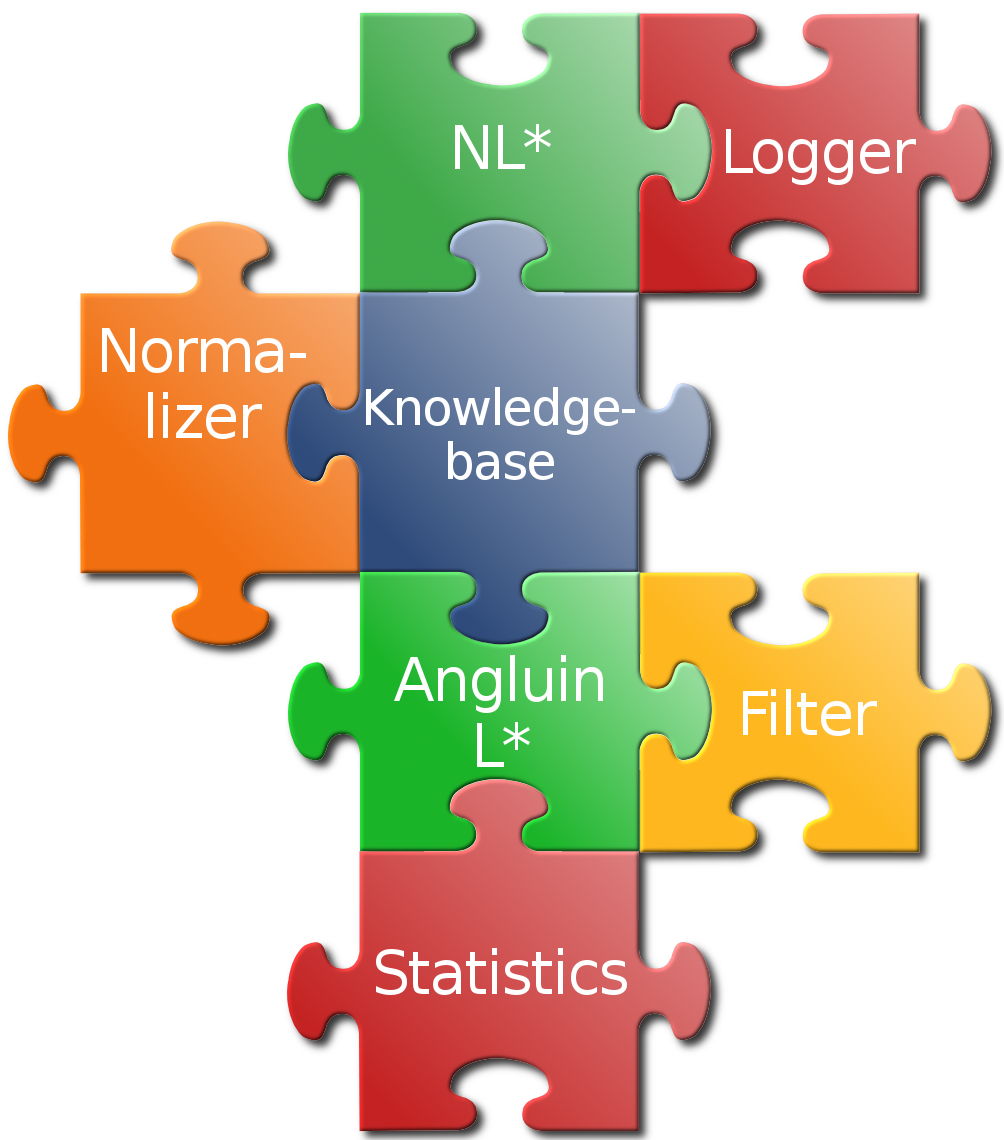
\includegraphics[width=0.5\textwidth]{images/combined6.png}
	\caption{Addition of Loggers and Statistics in Plug and Play fashion}
	\label{fig:loggers}
\end{figure}
	
\subsection{Connections of the Components}

The primary aspect in describing the working would be to outline the data flow between a learning algorithm, the knowledgebase and the user (or \emph{teacher}) as sketched in Figure \ref{communications}.

\begin{figure}
\centering
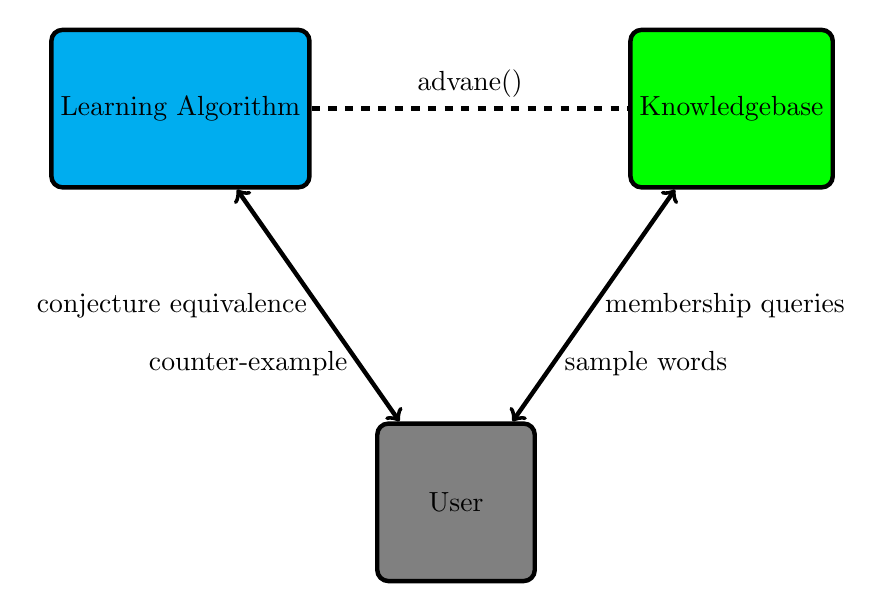
\begin{tikzpicture}[rounded corners,ultra thick]
\draw node[minimum height=2cm,minimum width=2cm,fill=cyan,draw] (la) at (0,5) {Learning Algorithm};
\draw node[minimum height=2cm,minimum width=2cm,fill=green,draw] (kn) at (7,5) {Knowledgebase};
\draw node[minimum height=2cm,minimum width=2cm,fill=gray,draw] (user) at (3.5,0) {User};
\draw[dashed,ultra thick] (la) -- (kn) node[midway,above] {advane()};
\draw[<->,ultra thick] (la) -- (user) node[midway,left] {conjecture equivalence} node[near end,left] {counter-example};
\draw[<->,ultra thick] (kn) -- (user) node[midway,right] {membership queries} node[near end,right] {sample words};
\end{tikzpicture}
\caption{data flow of the \libalf components}
\label{communications}
\end{figure}

	The learning algorithm and the knowledgebase share information with user. The knowledgebase, as stated earlier, is the fundamental information for the learning algorithm to develop an automaton. The learning algorithm advances with whatever knowledge is available. The learning algorithm connects with the user to collect relevant information such as equivalence of a conjecture or to retrive counter-example. When the learning algorithm creates more membership queries, they are stored in the knowledgebase leading to it initiating a communication with the user who is required to answer membership queries (or input sample words in case of an offline algorithm). All such information extended by the user are stored in the knowledgebase. 

\section{Demo Application}

In this section we describe the working of the \offline and \online algorithms with reference to the demo code in \cpp available at our website \url{http://libalf.informatik.rwth-aachen.de/}. Demo programs of the algorithms in \java are also available there.

The following code snippet briefly demonstrates how to employ the \libalf library in a user application. It is important that you become familiar with the auxilliary methods used in the program and hence their operations are explained first.

\begin{itemize}
\item \textbf{\emph{get\_AlphabetSize()}} - Promts the user to provide information about the size of alphabet and stores it as an \texttt{Integer}.
\item \textbf{\emph{answer\_Membership(\*li)}} - Takes the list of queries as an arguement and presents it to the user to classify them. It returns \texttt{true} when the word is to be accepted and returns \texttt{false} when it is to be rejected.
\item \textbf{\emph{check\_Equivalence(cj)}} - Presents the computed conjecture to the user who marks it as correct or incorrect. Returns \texttt{true} or \texttt{false} respectively.
\item \textbf{\emph{get\_CounterExample(alphabetsize)}} - Requests the user to input the counter-example and returns the word as a list (array in \java implementation) of integers. It takes the alphabetsize as a parameter for validation purposes.
\item \textbf{\emph{get\_Samples(alphabetsize)}} - Retrieves the sample word from the user. The alphabetsize is passed as a parameter for validation purposes.
\item \textbf{\emph{classification = get\_Classification()}} - Retrieves the classification of the sample word from the user. Returns \texttt{true} when the word is to be accepted and returns \texttt{false} when it is to be rejected.
\item \textbf{\emph{enough\_Samples()}} - Requests the user to specify whether all samples have been provided by the user. Returns ``y'' if user desires addition of more samples or ``n'' if all samples have been provided already.
\end{itemize}

\subsection{Online Algorithm}

An \online Algorithm, as mentioned in the previous section, formulates the conjecture by putting forth ``queries'' to the \teacher.

\lstset{language=c++, numbers=left, numberstyle=\tiny, stepnumber=1, numbersep=5pt}
\begin{lstlisting}[frame=single]
void main(int argc, char**argv) {
int alphabetsize = get_AlphabetSize();
knowledgebase<bool> base;
angluin_simple_table<bool> algorithm(&base,
NULL,alphabetsize);
do {
 conjecture * cj = algorithm.advance();
 if (cj == NULL) 
 {
   list<list<int> > queries = base.get_queries();
   list<list<int> >::iterator li;
   for(li = queries.begin(); li != queries.end(); li++) 
   {
      bool a = answer_Membership(*li);
      base.add_knowledge(*li, a);
   }
 }
 else 
 {
   bool is_equivalent = check_Equivalence(cj);
   if (is_equivalent) result = cj; 
   else 
   {	
      list<int> ce = get_CounterExample(alphabetsize);
      algorithm.add_counterexample(ce);
   }
 }
}while (result == NULL);
cout<<result->visualize();
}
\end{lstlisting}

The workflow of the program is as described below:

\begin{enumerate}
	\item At line 2, the program promts the user to input the \alphsize of the Automaton.
	\item An empty knowledgebase is now intialized at line 3. (The knowledgebase stores the words as a list of \texttt{Integers})
	\item Now, a learning algorithm is created by providing three parameters - the knowledgebase, NULL for a logger, the Alphabet Size.
	\item After having initialized the learning algorithm, the program is subjected to a loop where the algorithm is made to \advanced (Line 7). The result of this is stored in a \conjecture type variable \cj.
	
	\item If there was no sufficient information available in the knowledgebase to construct a conjecture, then \cj is NULL and the algorithm enters the condition at line 8. The algorithm produces the \memque that needs to be resolved by the user (or \teacher). The queries are obtained using the method \getqueries. (Note: the queries are obtained in ``list of list of \texttt{Integers}'' since words are stored as \texttt{Integers} and there may be more than one query)
	
	\item The queries produced are presented to the user who classifies it as \accepted or \rejected. This is done at Line 13 with \answer function. Subsequently, This information is added to the knowledgebase and the iteration of the loop continues.

	\item However, if a conjecture was computed at line 7, (implying that enough information was available in the knowledgebase), then algorithm enters the condition at line 18. The conjecture is presented to the user by \checkeq function at line 20.
	
	\item If the conjecture is equivalent, the user marks it correct and the conjecture is stored in variable \result. Iteration ends and the \result is displayed in line 32.
	
	\item If it is not equivalent, the user is now prompted to provide a counter example (line 27) and the program continues with the iteration. Typically, the counter example would influence the learning algorithm to invoke more \memque that is to be resolved during the next \advanced of the algorithm.
\end{enumerate}

\subsection{Offine Algorithm}

An \offline algorithm, as mentioned in the previous section, computes a conjecture from a set of passively provided input samples with their classifications.

\lstset{language=c++, numbers=left, numberstyle=\tiny, stepnumber=1, numbersep=5pt}
\begin{lstlisting}[frame=single]
int main(int argc, char**argv) 
{
  int alphabetsize = get_AlphabetSize();
  string input = "y";
  list<int> words;
  bool classification;
  knowledgebase<bool> base; 
  while (input == "y") 
  {
    words = get_Samples(alphabetsize);
    classification = get_Classification();
    base.add_knowledge(words, classification);
    input = enough_Samples();
  }
  RPNI<bool> algorithm(&base, NULL, alphabetsize);
  conjecture *cj = algorithm.advance();
  cout <<cj->visualize();
}
\end{lstlisting}

The workflow of the above program is as follows:

\begin{enumerate}

\item At line 2, the program prompts the user to input the \alphsize used for the automaton (coded in the function \getsize)
\item Variables for storing the sample words and their classifications are described subsequently. An empty knowledgebase is now initialized. 
\item The program then passes over a loop which recursively performs the action of reading the sample (line 10) and its classification (line 11) from the user. As and when the user inputs this information, it is continually added to the knowledgebase (line 13). The loop ends when the user indicates that the desired number of samples have been entered as coded in line 13 (its for this purpose that the \stringtype \inputs is first initialized to ``y'').
\item Now, a learning algorithm (RPNI Offline Algorithm) is created by providing three parameters - the knowledgebase, NULL for a logger, the Alphabet Size (line 15)
\item Having initialized the algorithm, it is now made to \advanced which produces a conjecture that pertains to the user's specification of samples. (line 16)
\item Finally, the conjecture is printed as coded in line 17 of the program.

\end{enumerate}

In both the command line programs implemented in \cpp and \java, the program outputs the ``.dot'' file which contains the code that builds the conjecture graphically. (This file may be executed using the GraphVIZ tool).


